% !TeX spellcheck = de_DE

\documentclass[12pt,a4paper,parskip=half]{scrreprt}

\usepackage[english]{babel}
\usepackage[utf8]{inputenc}
\usepackage{acronym}
\usepackage{graphicx}
\usepackage[below]{placeins}
\usepackage{url}
\usepackage{hyperref}
\usepackage{tabularx}
\usepackage{booktabs}
\usepackage{textcomp}
\usepackage{caption}

\newcommand{\source}[1]{\caption*{Source: {#1}} }

\title{Bericht Praxisphase I}
\author{Sebastian Wallat}
\date{\today}

\clubpenalty = 10000 % schliesst Schusterjungen aus
\widowpenalty = 10000 % schliesst Hurenkinder aus

\graphicspath{{./images/}}

\begin{document}

\begin{titlepage}
	
	\centering
	
%%	\ifcsempty{iodhbwm@institute@logo}{%
		
%%		
\includegraphics[height=1.5cm]{dhbw-logo}
		
	{%
		
		\begin{minipage}[c]{.25\textwidth}
			
			
\includegraphics[width=\textwidth, height = 2cm]{dhbw-logo}
			
		\end{minipage}
		\begin{minipage}[c]{0.46\textwidth}
			
			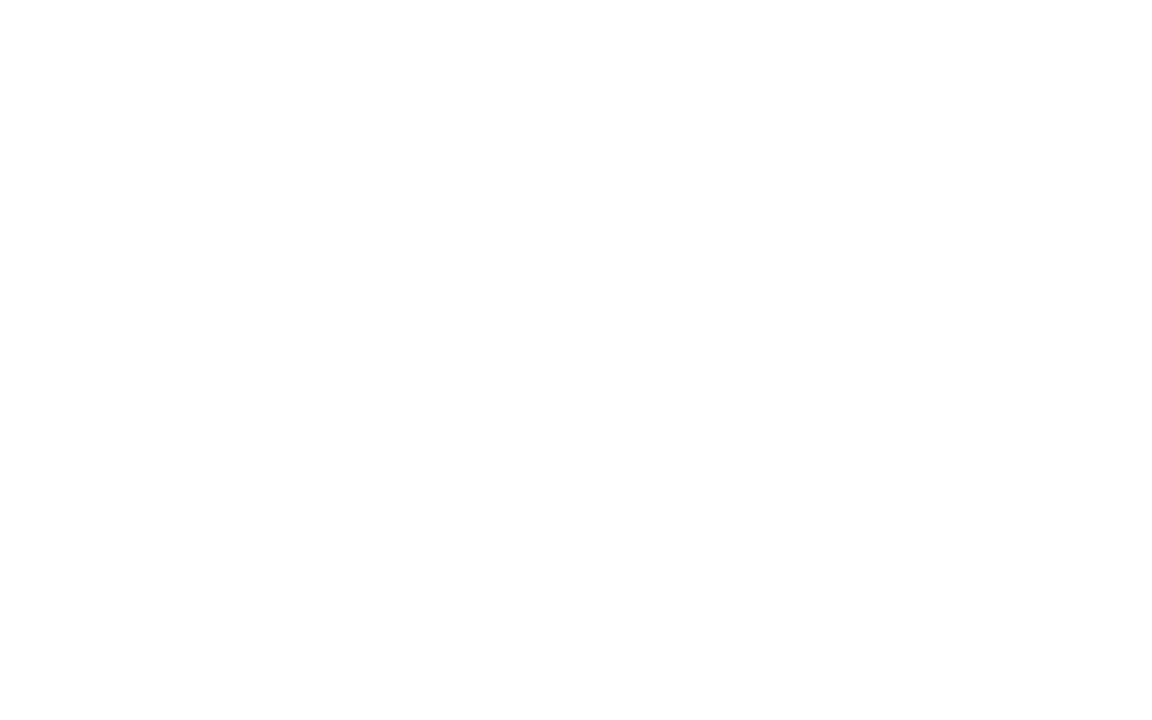
\includegraphics[width=\textwidth]{empty}
			
		\end{minipage}
		\begin{minipage}[c]{.25\textwidth}
			
			\raggedleft
			
			
\includegraphics[width=\textwidth, height =2cm, keepaspectratio]{dlr-logo}
			
		\end{minipage}
		
	}
	
	
	
	\bigskip
	
	
	
	\Large\textsc{Hausarbeit}
	
	
	
	\normalsize
	
	des Studiengangs Informationstechnik\par
	
	der Dualen Hochschule Baden-Württemberg Mannheim
	
	
	
	\rule{\textwidth}{.5mm}\bigskip
	
	
	
	\textsc{\large Sicherheit und Fehlermodelle von verteilten Systemen}	
	
	
	\rule{\textwidth}{.5mm}
	
	
	
	\vfill
	
	
	
	\par
	
	{\bfseries\large Julian Fuchs, Marius Bröcker, Sebastian Wallat}\par
	
	\today
	
	
	
	\vfill
	
	
	
	\small{%
		
		\begin{tabularx}{\textwidth}{@{}lX@{}}
			
			\toprule
			
			
			Bearbeitungszeitraum: & 24.10.2020-27.11.2020\\
			
			Matrikelnummer, Kurs: & 1708267, TINF18-IT1\\
			
			Vorlesung: & Verteilte Systeme \\
			
		\end{tabularx}
		
	}
	
	\cleardoublepage
	
\end{titlepage}


\newpage
\pagenumbering{Roman}

\chapter*{Eidesstattliche Erklärung}
%%\thispagestyle{empty}
\vspace{50pt}
Wir versichern hiermit, dass wir diese Hausarbeit mit dem Thema: ''Sicherheit und Fehlermodelle von verteilten Systemen'' selbständig verfasst und keine anderen als die angegebenen Quellen und Hilfsmittel benutzt haben.
\\
\\

\vfill
\noindent\rule{5cm}{.4pt}\hfill\rule{5cm}{.4pt}\par
\noindent Datum, Ort \hfill Unterschrift 

\newpage
\thispagestyle{empty}
\chapter*{Zusammenfassung}

Thema
\\
\bigskip

\tableofcontents
\addtocontents{toc}{}

\listoffigures
\addcontentsline{toc}{chapter}{Abbildungsverzeichnis} 
%%\thispagestyle{empty}

\newpage
\chapter*{Abkürzungsverzeichnis}
\addcontentsline{toc}{chapter}{Abkürzungsverzeichnis}
%%\thispagestyle{empty}
\begin{acronym}[HTTP]
	\acro{DLR}{\textbf{D}eutsches Zentrum für \textbf{L}uft- und \textbf{R}aumfahrt}
\end{acronym}

\pagenumbering{arabic}

\chapter{Einführung}

Ein wichtiger Aspekt verteilter Systeme (vS) ist das erhöhte Sicherheits- und Schutzbedürfnis dieser. Dies ergibt sich aus ihrem offenen Aufbau, sowie der netzwerkgestützten Kommunikation zwischen den einzelnen Teilsystemen. Aus diesem Grund besitzen verteilte Systeme eine viel zahl verschiedenster Angriffsvektoren. Besonders im Kontext von kritischer Infrastruktur (KRITIS) und verschiedenen Branchen wie etwa Banken und E-Commerce müssen Sicherheit und Datenschutz als essentielle Bestandteile des Gesamtsysteme angesehen werden.
\\
Um eine möglichst große Zahl an möglichen Sicherheitsproblemen zu eliminieren ist es notwendig schon während der ersten Planungsphasen die sicherheitsrelevanten Aspekte mit in die Überlegungen einzubeziehen. So können eventuelle Schwachstellen möglichst früh identifiziert und entsprechende Gegenmaßnamen in das System integriert werden. Wichtig hierbei ist das alle Schutzmaßnamen kontinuierlich im gesamten System implementiert werden, da schon eine einziger Mangel innerhalb einer Komponente zur Kompromittierung des Gesamtsystems führen kann.
\\
Um allen Sicherheits- und Datenschutz relevanten Anforderungen modernen IT Systeme zu entsprechen sind eine viel zahl verschiedenster Mechanismen und Sub-Komponenten zu betrachten. Die wichtigsten dieser sollen im weiteren Verlauf dieser Arbeit näher beleuchtet werden, hierzu zählen unter anderem:

\begin{itemize}
	\item Kryptoverfahren
	\item Authentisierung
	\item Autorisierung
	\item Arten von Fehlern und Störungen, sowie deren korrekte Behandlung
\end{itemize}


\chapter{Sicherheit}


\section{Schutzziele}

An dieser Stelle lohnt es sich kurz auf die Grundlagen der Informationssicherheit IT-Sicherheit einzugehen.
\\
\\
''Als Informationssicherheit bezeichnet man Eigenschaften von informationsverarbeitenden und -lagernden (technischen oder nicht-technischen) Systemen, die die
Schutzziele Vertraulichkeit, Verfügbarkeit und Integrität sicherstellen.
Informationssicherheit dient dem Schutz vor Gefahren bzw. Bedrohungen, der Vermeidung von wirtschaftlichen Schäden und der Minimierung von Risiken.''[\cite{ScriptITSicherheit}]
\\
''IT-Sicherheit ist ein Teil der Informationssicherheit. In Abgrenzung zur IT-Sicherheit umfasst die
Informationssicherheit neben der Sicherheit der IT-Systeme und der darin gespeicherten Daten auch noch die Sicherheit von nicht elektronisch verarbeiteten Informationen.''[\cite{ScriptITSicherheit}]
\\
\\
Somit lässt sich festhalten, das die Schutzziele Vertraulichkeit, Verfügbarkeit und Integrität die oberste Priorität aller Sicherheitstechnischen Überlegungen darstellen sollten. Im folgenden sollen diese drei Schutzziele weiter erläutert werden:

\begin{itemize}
	\item Vertraulichkeit: Verhinderung von jeglichen unautorisierter Informationsgewinn (Abgreifen von vertraulichen Daten)
	\item Integrität: Verhinderung von unabsichtlicher bzw. unautorisierter Modifizierung von Daten. (Falls eine Datenveränderung nicht komplett unterbunden werden kann, so muss zumindest gewährleistet werden, dass diese vom System bemerkt wird)
	\item Verfügbarkeit: Es muss verhinder werden, dass autorisierte Subjekte von unautorisierten Zugriffen in der Nutzung ihrer Berechtigungen beeinträchtigt werden.
\end{itemize}


\section{Angriffsvektoren}

Ziel eines möglichen Angreifers ist es, eines der im vorherigen Kapitel erläuterten Schutzziele zu verletzen. Hierbei kann ein bestimmter Angriff (Vektor) durchaus mehrere Schutzziele kompromittieren. Im folgenden sollen einige mögliche Angriffsmöglichkeiten beispielhaft aufgeführt werden.

\begin{itemize}
	\item Man-in-the-Middle(MITM): Vertraulichkeit
	\item Trojaner (z.B. Emotet/Trickbot): Integrität
	\item Denial of Service (Dos/DDos): Verfügbarkeit
	\item SQL-Injection: Vertraulichkeit, Integrität
\end{itemize}


\section{Schutzmaßnahmen}


\subsection{Verschlüsselung}


\subsection{Authentisierung}


\subsection{Autorisierung}


\chapter{Fehlermodelle}


\section{Anforderungen}


\section{Arten von Fehlern und Störungen}


\section{Fehlerbehebung}


\newpage

\nocite{*}
\thispagestyle{headings}

\bibliographystyle{IEEEtr}
\bibliography{bibo} 


\end{document}